\section{Experiments}

\subsection{Benchmark}

Our experimental evaluation utilizes TheAgentCompany (TAC) benchmark~\citep{xu2024theagentcompanybenchmarkingllmagents}. Comprising 175 tasks, this benchmark is designed to assess the comprehensive capabilities of autonomous language agents by simulating a high-fidelity corporate environment. The tasks are structured around six core employee positions (e.g., HR, PM, SDE), requiring the agent to execute interconnected operations using a suite of applications such as chat clients, cloud storage, and project management software, all within a fully functional operating system.
A core feature of TAC is the high complexity and long-horizon nature of its tasks. On average, completing a task requires over 40 action steps, frequently spanning two or more applications. This demands that an agent decompose high-level objectives into a coherent, protracted sequence of steps and integrate information across platforms. Therefore,  TAC provides a rigorous platform for evaluating an agent's real-world problem-solving, multi-step planning, and long-horizon reasoning capabilities, making it highly suitable for our research focus on long-horizon productivity tasks.


\subsection{Experimental Setup}
\label{sec:ex_setup}

In our experimental configuration, the PE Agent and Reflect Agent employ the Gemini-2.5 Flash model~\citep{comanici2025gemini}, while NPCs in the TAC environment are powered by GPT-4o model. The maximum number of actions for each sub-task is set to $N=20$. For evaluation, we rely on the official protocol provided by the TAC benchmark. This evaluation protocol not only assesses the final completion status of a task but also defines a series of critical intermediate checkpoints to measure partial progress. The primary metric is the partial completion score ($S_{partial}$), which is calculated as:
$S_{partial} = 0.5 \cdot {\text{Completed\_ckpt}} / {\text{Total\_ckpt}} + 0.5 \cdot S_{full}$,
where $S_{full} \in \{0,1\}$ is a binary indicator of whether the task was fully completed. Our final performance metric is computed as the average partial completion score across all evaluated tasks. Additionally, we calculate an aggregate checkpoint score, $S_{ckpt}$, which represents the proportion of completed checkpoints relative to the total checkpoints across all tasks.

\subsection{Experimental Results}
\subsubsection{Continuous Learning Experiments}

To validate the continual learning capability of our {\method} framework, we curated a subset of 18 tasks from TAC benchmark, which we denote as $\mathcal{T}_{cl}$. This subset was sampled to ensure coverage across all six professional roles. Our experimental design simulates how humans accumulate experience, with the primary objective of testing whether the agent can progressively improve its performance on repetitive tasks by continuously updating its memory. For comparison, we first establish a baseline by evaluating the Gemini-2.5 Flash model on $\mathcal{T}_{cl}$ without our Memory Module. The main experiment then consists of three sequential iterations with no human intervention, where in each iteration, the agent tackles all 18 tasks in order, carrying its accumulated knowledge forward to the next. To mitigate randomness, we conduct five complete runs of this experiment and report the average scores. 
The detailed tasks in $\mathcal{T}_{cl}$ are elaborated in \Cref{app:task_split} and \Cref{tab:task_sets}.
% The results are presented in Figure~\ref{fig:cl_plot}. 

\begin{wrapfigure}[18]{!t}{0.5\textwidth} 
    \centering
    \vspace{-10pt}
    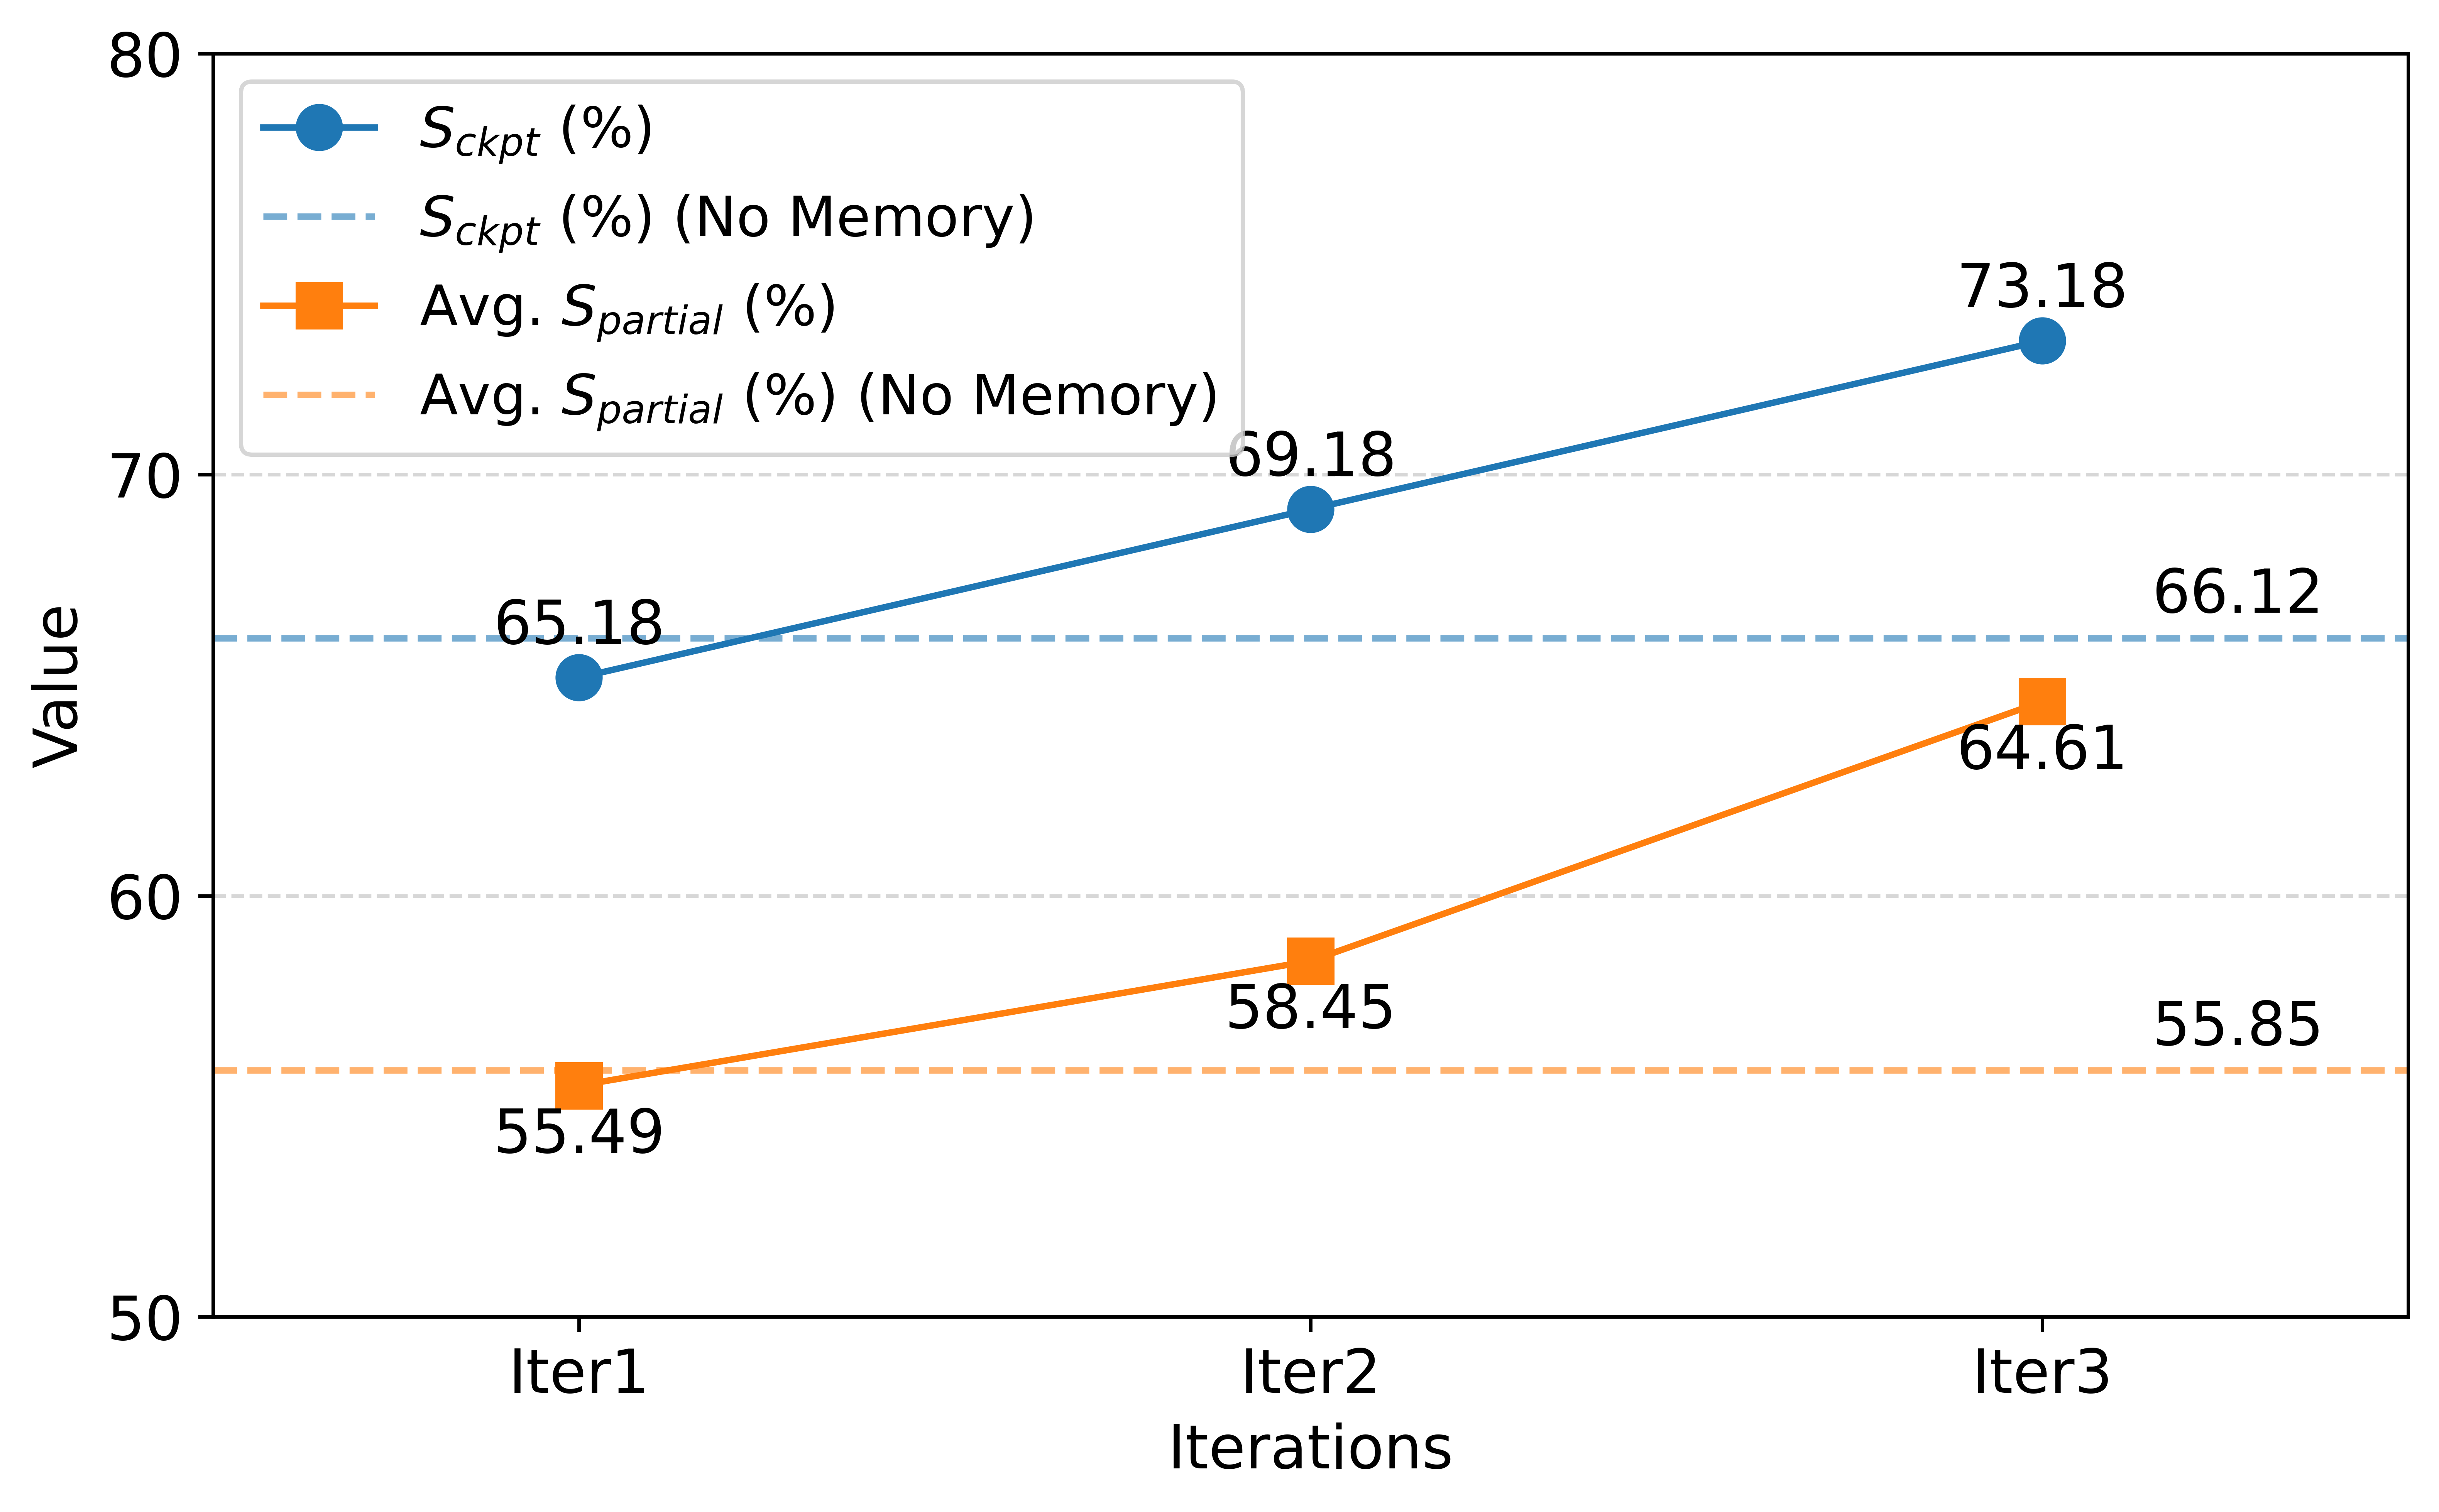
\includegraphics[width=\linewidth]{figures/cl_plot.png}
    \vspace{-10pt}
    \caption{Performance trends across iterations of {\method}. 
The figure shows $S_{ckpt}$ (blue) and average $S_{partial}$ (orange). 
Dashed lines denote the baseline without memory, while solid lines track improvements across iterations.}
    \label{fig:cl_plot}
\end{wrapfigure}


As illustrated in Figure~\ref{fig:cl_plot}, the results clearly show that both the $S_{ckpt}$ and $S_{partial}$ metrics grew steadily and monotonically across the three iterations, a direct manifestation of our framework's self-evolving capability. Most critically, in the final round, {\method} outperformed the memory-less baseline by over 10\%, confirming the effective translation of self-accumulated knowledge into substantial performance gains. We attribute this advantage to the accumulated experience, which enables the agent to avoid previously failed exploration paths and thus focus more directly on effective solutions. This approach not only improves efficiency by streamlining the LLM's context but also enables the agent to achieve an unprecedented depth of exploration.

\subsubsection{Generalization Experiments}

To further evaluate the generalization capability of our memory mechanism, we curate a challenging subset from the TAC benchmark, denoted as $\mathcal{T}_{hard}$. This subset comprises 12 tasks on which even strong models like Claude-4 Sonnet achieve little to no score. The purpose of this experiment is to test our agent's zero-shot generalization ability when facing entirely new and highly difficult tasks. 
Specifically, we compare a baseline agent operating without memory against our agent equipped with the fixed Memory Module, which is accumulated over three iterations of continual learning on the $\mathcal{T}_{cl}$ set. Both agents are evaluated on this previously unseen $\mathcal{T}_{hard}$ task set. By comparing their performance differences, we can easily determine whether the memory mechanism can effectively transfer historical experience to unknown scenarios. Detailed $\mathcal{T}_{hard}$ are elaborated in \Cref{app:task_split}.

\begin{table}[t]
\centering
\small
\caption{Performance comparison on the hard-task set. The agent with memory demonstrates significant improvement.}
\vspace{5pt}
\label{tab:hard}
\begin{tabular}{ll|ccc}
\toprule
Framework & Model & checkpoint & $S_{ckpt}$ (\%) $\uparrow$ & Avg. $S_{partial}$ (\%) $\uparrow$\\
\midrule
% {\method} w/o mem  & 22 / 59 & 37.3 & 27.0 \\
Openhands-versa~\citep{soni2025codingagentsmultimodalbrowsing} & claude-4 sonnet & 3 / 59 & 5.08 & 2.00 \\
Openhands~\citep{wang2024openhands} & gemini-2.5 pro & 5 / 59 & 8.47 & 3.00 \\
{\method} w/o mem & gemini-2.5 flash & 18 / 59 & 30.51 & 23.65 \\
{\method} w/ mem & gemini-2.5 flash  & \textbf{24 / 59} & \textbf{40.68} & \textbf{33.41} \\
\bottomrule
\end{tabular}
\vspace{-10pt}
\end{table}


As shown in Table~\ref{tab:hard}, current SOTA agents, such as the Openhands framework~\citep{wang2024openhands} using powerful closed-source models like Gemini-2.5 Pro~\citep{comanici2025gemini} and Claude-4 Sonnet~\citep{anthropic2025claude4}, struggle significantly on $\mathcal{T}_{hard}$. In general, they complete fewer than 10\% of the checkpoints and achieve an $S_{partial}$ of only 2\% or 3\%. In contrast, our {\method}, using only the lighter Gemini-2.5 Flash model, reaches an $S_{partial}$ of 23.65\% even without relying on memory, which demonstrates the effectiveness of the synergy between our PE and Reflect Agents. When equipped with its pre-learned memory, our agent's performance further improves to a remarkable $S_{partial}$ of 33.41\%. This result provides strong evidence for the zero-shot generalization capability of the knowledge acquired through our framework, indicating that {\method} learns transferable and generalizable memory, rather than merely remembering task-specific solutions.


\subsubsection{TAC Full Benchmark}
\label{sec:full tac}

To conduct a fair and comprehensive comparison against other leading agent methods, we evaluated our framework on the complete TAC benchmark, which includes all 175 tasks. For this experiment, the agent was equipped with the Memory Module accumulated after three iterations on the $\mathcal{T}_{cl}$ subset, and this memory was kept frozen throughout the evaluation.

As shown in Table~\ref{tab:full}, {\method} achieves new SOTA performance on the TAC benchmark. Notably, it attains an average $S_{partial}$ of 51.78\%, marking the first time an agent has surpassed the 50\% threshold on this benchmark and outperforming the previous SOTA (OpenHands-versa w/ Claude-4 Sonnet) by nearly 20\%. This substantial improvement is particularly striking given that our agent's memory was acquired from only approximately 10\% of the available tasks, demonstrating exceptional ``learning on the job'' efficiency. These results prove the effectiveness of {\method} in challenging real-world productivity tasks. Besides, they provide strong empirical support for our core thesis: past condensed experience yields highly generalizable capabilities that far exceed what might be expected from the limited learning.
The complete results of 175 tasks are listed in \Cref{tab:full_detail}. 

\begin{table}[h]
\centering
\small
% \vspace{-10pt}
\setlength{\tabcolsep}{1.5pt}
\caption{Performance comparison across frameworks and models on the TAC full 175-task benchmark. 
\textbf{PCR} (Perfect Completion Rate) indicates the proportion of tasks that are fully solved.}
% \vspace{5pt}
\label{tab:full}
\begin{tabular}{ll|cccccc}
\toprule
Framework & Model & checkpoint & $S_{ckpt}(\%)\uparrow$ & Avg. $S_{partial}(\%)\uparrow$ & PCR(\%)$\uparrow$ \\
\midrule
\multirow{1}{*}{OWL-RolePlay~\citep{hu2025owl}}     
  & gpt-4o + o3-mini  & 127 / 776 & 16.37 & 11.04 & 4.00 \\
\midrule
\multirow{3}{*}{Openhands~\citep{wang2024openhands}} 
  & gemini-1.5 pro & 90 / 776 & 11.60 & 8.02 & 3.43 \\
  & gemini-2.0 flash & 195 / 776 & 25.13 & 18.96 & 11.43 \\
  & gemini-2.5 pro   & 361 / 776 & 46.52 & 39.28 & 30.29 \\
\midrule
\multirow{2}{*}{Openhands-Versa~\citep{soni2025codingagentsmultimodalbrowsing}} 
  & claude-3.7 sonnet  & 353 / 776 & 45.49 & 40.18 & 30.86 \\
  & claude-4 sonnet  & 392 / 776 & 50.52 & 43.19 & 33.14 \\
\midrule
% \rowcolor{grey!20} 
\multirow{1}{*}{\method~~(ours)}   & gemini-2.5 flash & \textbf{465 / 776} & \textbf{59.92} & \textbf{51.78} & \textbf{41.14} \\
\bottomrule
\end{tabular}
\end{table}

\subsection{Ablation Study}
\subsubsection{Ablation Study for Reflect Agent}

To evaluate the impact of the Reflect Agent in the {\method} framework, we conduct an ablation study by removing it. Specifically, we compare a variant lacking the Reflect Agent against the full framework, with both configurations operating without the Memory Module. As presented in Table~\ref{tab:reflection}, the non-reflective variant underperformed on the 18-task subset $\mathcal{T}_{cl}$. This result demonstrates the indispensable role of the reflective mechanism in ensuring execution quality and providing the high-quality signal required for effective learning.

\begin{table}[h]
\centering
\small
% \vspace{-10pt}
\caption{Performance comparison of ablation studies of Reflect Agent on $\mathcal{T}_{cl}$.
Results show that removing the Reflect Agent (\emph{No Reflection Variant}) leads to a substantial performance drop.}
% \vspace{5pt}
\label{tab:reflection}
\begin{tabular}{ll|ccc}
\toprule
Framework  & Model & checkpoint & $S_{ckpt}$ (\%) $\uparrow$ & Avg. $S_{partial}$ (\%) $\uparrow$ \\
\midrule
No Reflection Variant & gemini-2.5 flash  & 54 / 85 & 63.53 & 43.21 \\
{\method} & gemini-2.5 flash & \textbf{56.2 / 85} & \textbf{66.12} & \textbf{55.85} \\
\bottomrule
\end{tabular}
\end{table}

\subsubsection{Ablation Study for Different Models}

To evaluate the open-source LLM adaptability of our framework, we replace the core model with DeepSeek-V3-250324~\citep{liu2024deepseek} and conduct experiments in two scenarios: with and without the pre-accumulated memory. 
The results, when compared against other open-source-based agents in Table~\ref{tab:open}, yield two key insights. First, even without memory, the {\method} architecture alone enables DeepSeek-V3 to outperform all other frameworks using open-source models, highlighting the intrinsic advantages of our design. Second, the addition of the pre-accumulated Memory Module provides a significant performance boost, confirming that our memory mechanism is model-agnostic and that the accumulated knowledge can be effectively transferred across different LLMs.

\begin{table}[h]
\centering
\small
% \vspace{-10pt}
\caption{Performance comparison of agents utilizing open-source LLMs on $\mathcal{T}_{cl}$.}
% \vspace{5pt}
\label{tab:open}
\begin{tabular}{ll|cccc}
\toprule
Framework & Model & checkpoint & $S_{ckpt}$ (\%) & Avg. $S_{partial}$ (\%) \\
\midrule
\multirow{3}{*}{Openhands} 
  & llama-3.1 405b & 17 / 85 & 20.00 & 9.78    \\
  & llama-3.3 70b & 11 / 85 & 12.94 & 5.84 \\
  & qwen-2.5 72b & 11 / 85 & 12.94 & 6.50 \\
\midrule
\multirow{1}{*}{{\method} w/o memory} 
  & deepseek-v3 & 29 / 85 & 34.12 & 28.01 \\
\multirow{1}{*}{{\method} w memory} 
  & deepseek-v3 & \textbf{43 / 85} & \textbf{50.59} & \textbf{36.75} \\
\bottomrule
\end{tabular}
\vspace{-10pt}
\end{table}